\section{Analyse empirique de l'auto-complétion}
Nous avons fixé $k=20$ et mesuré le temps moyen de \texttt{acComplete} sur 100 essais pour des longueurs de requête $l$ allant de 0 à 10.


\begin{itemize}
    \item MergeSort
    \item QuickSort
    \item PQ + MergeSort
    \item PQ + QuickSort
\end{itemize}

\subsection{Dataset: actors\_25k}

\begin{center}
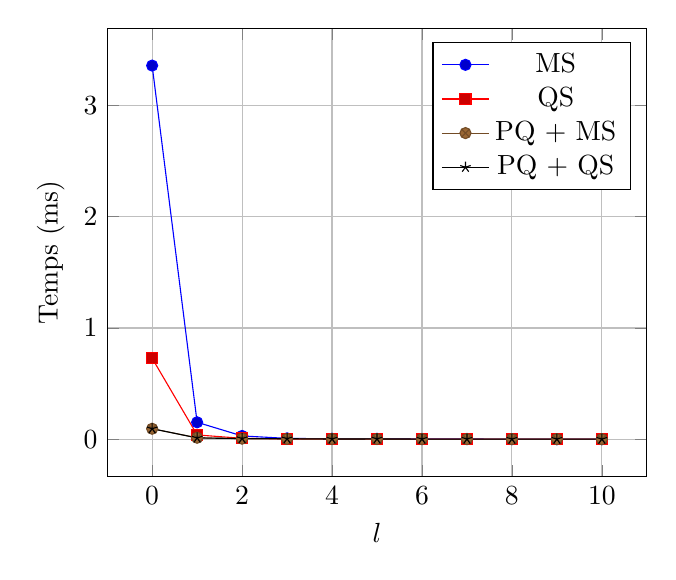
\begin{tikzpicture}
\begin{axis}[
    xlabel={$l$},
    ylabel={Temps (ms)},
    legend pos=north east,
    grid=both
]

\addplot coordinates {
(0,3.357140)(1,0.152920)(2,0.030380)(3,0.008470)(4,0.004670)
(5,0.004130)(6,0.002650)(7,0.002790)(8,0.001690)(9,0.001340)(10,0.001420)
};
\addlegendentry{MS}

\addplot coordinates {
(0,0.727970)(1,0.039380)(2,0.008900)(3,0.003320)(4,0.002320)
(5,0.002090)(6,0.001740)(7,0.001490)(8,0.001420)(9,0.001440)(10,0.001200)
};
\addlegendentry{QS}

\addplot coordinates {
(0,0.094910)(1,0.014040)(2,0.005860)(3,0.003570)(4,0.002860)
(5,0.002540)(6,0.002000)(7,0.001850)(8,0.001570)(9,0.001470)(10,0.001190)
};
\addlegendentry{PQ + MS}

\addplot coordinates {
(0,0.095240)(1,0.012350)(2,0.006810)(3,0.005240)(4,0.002870)
(5,0.003510)(6,0.002000)(7,0.002170)(8,0.001840)(9,0.001820)(10,0.001730)
};
\addlegendentry{PQ + QS}

\end{axis}
\end{tikzpicture}
\end{center}

\subsection{Dataset: actors\_250k}

\begin{center}
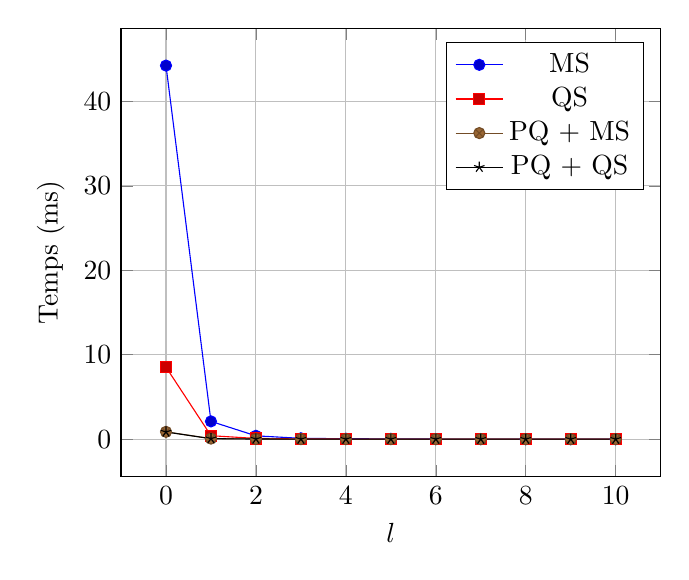
\begin{tikzpicture}
\begin{axis}[
    xlabel={$l$},
    ylabel={Temps (ms)},
    legend pos=north east,
    grid=both
]

\addplot coordinates {
(0,44.248120)(1,2.110630)(2,0.400670)(3,0.105700)(4,0.055490)
(5,0.040900)(6,0.016530)(7,0.011540)(8,0.009180)(9,0.002900)(10,0.002120)
};
\addlegendentry{MS}

\addplot coordinates {
(0,8.536270)(1,0.415590)(2,0.092540)(3,0.031310)(4,0.018640)
(5,0.010630)(6,0.008520)(7,0.004760)(8,0.003440)(9,0.002470)(10,0.002060)
};
\addlegendentry{QS}

\addplot coordinates {
(0,0.872920)(1,0.072340)(2,0.024880)(3,0.010480)(4,0.008970)
(5,0.006260)(6,0.004810)(7,0.004390)(8,0.002950)(9,0.002120)(10,0.002330)
};
\addlegendentry{PQ + MS}

\addplot coordinates {
(0,0.854800)(1,0.060870)(2,0.022010)(3,0.010130)(4,0.007410)
(5,0.006430)(6,0.004850)(7,0.003620)(8,0.002680)(9,0.002360)(10,0.002140)
};
\addlegendentry{PQ + QS}

\end{axis}
\end{tikzpicture}
\end{center}

\subsection{Dataset: actors\_2500k}

\begin{center}
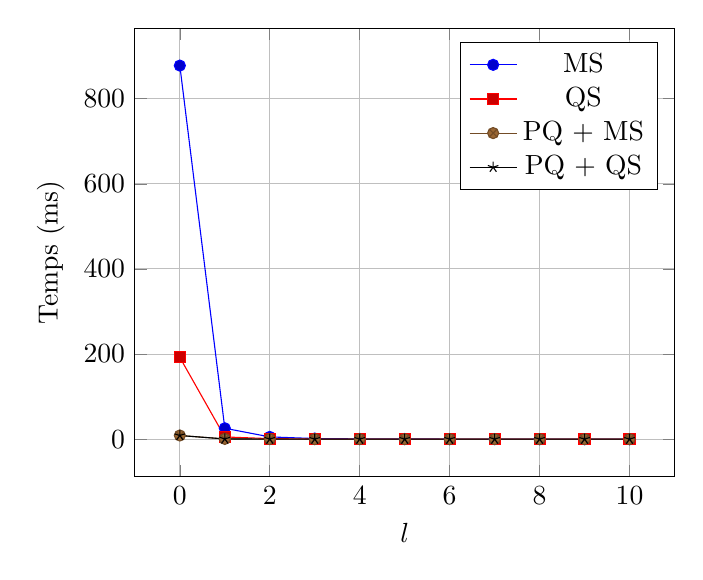
\begin{tikzpicture}
\begin{axis}[
    xlabel={$l$},
    ylabel={Temps (ms)},
    legend pos=north east,
    grid=both
]

\addplot coordinates {
(0,877.853000)(1,25.658830)(2,5.350360)(3,1.457220)(4,0.650860)
(5,0.476540)(6,0.219410)(7,0.132320)(8,0.072300)(9,0.040980)(10,0.016060)
};
\addlegendentry{MS}

\addplot coordinates {
(0,192.126730)(1,5.253260)(2,1.278010)(3,0.292890)(4,0.137000)
(5,0.136000)(6,0.086580)(7,0.026350)(8,0.015290)(9,0.008930)(10,0.004830)
};
\addlegendentry{QS}

\addplot coordinates {
(0,8.683540)(1,0.622170)(2,0.149790)(3,0.052060)(4,0.027950)
(5,0.021510)(6,0.011530)(7,0.009410)(8,0.007820)(9,0.004620)(10,0.003610)
};
\addlegendentry{PQ + MS}

\addplot coordinates {
(0,8.572070)(1,0.496540)(2,0.130880)(3,0.051660)(4,0.029350)
(5,0.020650)(6,0.016070)(7,0.010190)(8,0.005840)(9,0.005200)(10,0.003750)
};
\addlegendentry{PQ + QS}

\end{axis}
\end{tikzpicture}
\end{center}
